\documentclass[11pt,a4paper]{article}
\usepackage[utf8]{inputenc}
\usepackage[T1]{fontenc}
\usepackage{amsmath}
\usepackage{amsfonts}
\usepackage[scale = 0.82]{geometry}
\usepackage{amssymb}
\usepackage{graphicx}
\usepackage{pdfpages}
\usepackage[hidelinks]{hyperref}
\usepackage[round]{natbib}
\bibliographystyle{unsrtnat}
\usepackage{url}

%\bibliographystyle{alpha}

\usepackage{float}
\usepackage{subfig}
\usepackage{comment}
%\setlength{\parindent}{0pt}
%\title{Melting or dissolving of vertical ice face into saline water}
%\author{Yao Gahounzo\\[1cm]{\small Advisor: Dr. Michal Kopera}}

% insert month and year of your thesis, only:
\date{October 4, 2021}

\begin{document}
	
	%\maketitle
	
	\begin{titlepage} % Suppresses displaying the page number on the title page and the subsequent page counts as page 1
	\newcommand{\HRule}{\rule{\linewidth}{0.5mm}} % Defines a new command for horizontal lines, change thickness here
	
	%\center % Centre everything on the page
	\begin{center}
	%------------------------------------------------
	%	Headings
	%------------------------------------------------
	
	\textsc{\LARGE BOISE STATE UNIVERSITY}\\[1.5cm] % Main heading such as the name of your university/college
	
	\textsc{\Large Computing PhD}\\[0.5cm] % Major heading such as course name
	
	\textsc{\large Computational Math Science and Engineering}\\[0.5cm] % Minor heading such as cours title
	
	\textsc{\large Comprehensive Exam Synthesis paper}\\[2cm]
	
	%------------------------------------------------
	%	Title
	%------------------------------------------------
	
	\HRule\\[0.4cm]
	
	{\huge\bfseries Mathematical and numerical modeling of ice-ocean interface}\\[0.4cm] % Title of your document
	
	\HRule\\[1.5cm]
	
	%------------------------------------------------
	%	Author(s)
	%------------------------------------------------
	
	\begin{minipage}{0.4\textwidth}
		\begin{flushleft}
			\large
			\textit{Student}\\
			Yao \textsc{Gahounzo} % Your name
		\end{flushleft}
	\end{minipage}
	~
	\begin{minipage}{0.4\textwidth}
		\begin{flushright}
			\large
			\textit{Advisor}\\
			Dr. Michal \textsc{Kopera} % Supervisor's name
		\end{flushright}
	\end{minipage}
	
	%------------------------------------------------
	%	Date
	%------------------------------------------------
	\vfill
	\end{center} 
	\begin{center}
	    \textsc{\large Committee members}\\ [0.3cm]
	    
	%    Dr. Donna Calhoun \\
	%    Dr. Ellyn Enderlin \\
	%    Dr. Uwe Kaiser
	\end{center}
	
	\hspace{6cm}Dr. Donna Calhoun \par
	\hspace{6cm}Dr. Ellyn Enderlin \par 
	\hspace{6cm}Dr. Uwe Kaiser
	
	\vfill\vfill\vfill % Position the date 3/4 down the remaining page
	
	\center 
	{\large\today} % Date, change the \today to a set date if you want to be precise
	
	%------------------------------------------------
	%	Logo
	%------------------------------------------------
	
	%\vfill\vfill
	%\includegraphics[width=0.2\textwidth]{placeholder.jpg}\\[1cm] % Include a department/university logo - this will require the graphicx package
	 
	%----------------------------------------------------------------------------------------
	
	\vfill % Push the date up 1/4 of the remaining page
	
    \end{titlepage}
	
	\section{Introduction}
	
	The Antarctic and Greenland ice sheets and glaciers are the important components of the global climate system. Over the past decades, the anthropogenic forces due to human activities have caused the atmosphere and the ocean to warm \citep{noble2020sensitivity}; as a result, its leads to mass loss in the global ice sheets, glaciers, and sea ice. According to \cite{straneo2013north}, the mass loss from the Greenland ice sheets quadrupled over the past two decades, contributing to the observed global sea-level rise about of one quarter. Observations now indicate that the impact of the Greenland ice sheet mass loss goes beyond sea-level rise to include changes in ocean properties and circulation, nutrient and sediment transport, and ecosystem function \citep{catania2020future}. \cite{straneo2013north} found that the Greenland ice loss contribution to the sea level is twice that from the Antarctic ice sheets; this ice loss increased due to both increased surface melting and ice/glaciers discharge to the ocean. %, resulted from the acceleration, thinning and retreat of multiple marine-terminating glaciers.
	%The authors also found that the contribution of Greenland ice loss to sea level is twice that of the Antarctic ice sheets. This ice loss has increased due to increased surface melt and ice/glacier discharge to the ocean, resulting from accelerated thinning and retreat of several sea-terminating glaciers. 
	The latter is attributed to the acceleration of ice flow and thinning of fast-flowing marine-terminating outlet glaciers \citep{nick2013future}. Although outlet glaciers extend far into the ice sheet's interior, much work has focused on the terminal boundary at the ocean, as this is where changes in mass balance have been most significant. The Widespread changes in surface melt and ice flow indicate a response to external forcings and are consistent with observations of atmospheric and oceanic warming over and around Greenland \citep{bersch2007recent,box2009greenland,straneo2013north}. Changes in precipitation and increasing air temperatures are the external forcings that have led to increased surface melting of the ice sheet \citep{van2009partitioning,straneo2013north}. However, the processes behind the increased ice discharge remain elusive. %The acceleration of the glaciers is a result of the initial retreat of the marine terminations that decreased the flow resistance of the ice \citep{nick2009large}.
	Acceleration of glaciers results from the initial retreat of marine termini that decreased ice flow resistance, increased calving and thinning, and led to further retreat \citep{nick2009large,straneo2013challenges}. The central hypothesis supporting initial glacier retreat involves increased submarine melting of the ice-ocean interface \citep{straneo2013challenges}. Ocean-related reduction of Greenland glacier calving faces have been observed over the past two decades (e.g., \cite{rignot2010rapid,straneo2015dynamics,schaffer2017warm}). Progress has been made through field observations, modeling, and theoretical studies to understand the mechanisms of ice-ocean interaction and examine the plausibility of the hypothesis. However, the question regarding the submarine melting remains, as the field observation are limited.
	
	\begin{figure}[H]
	    \centering 
	    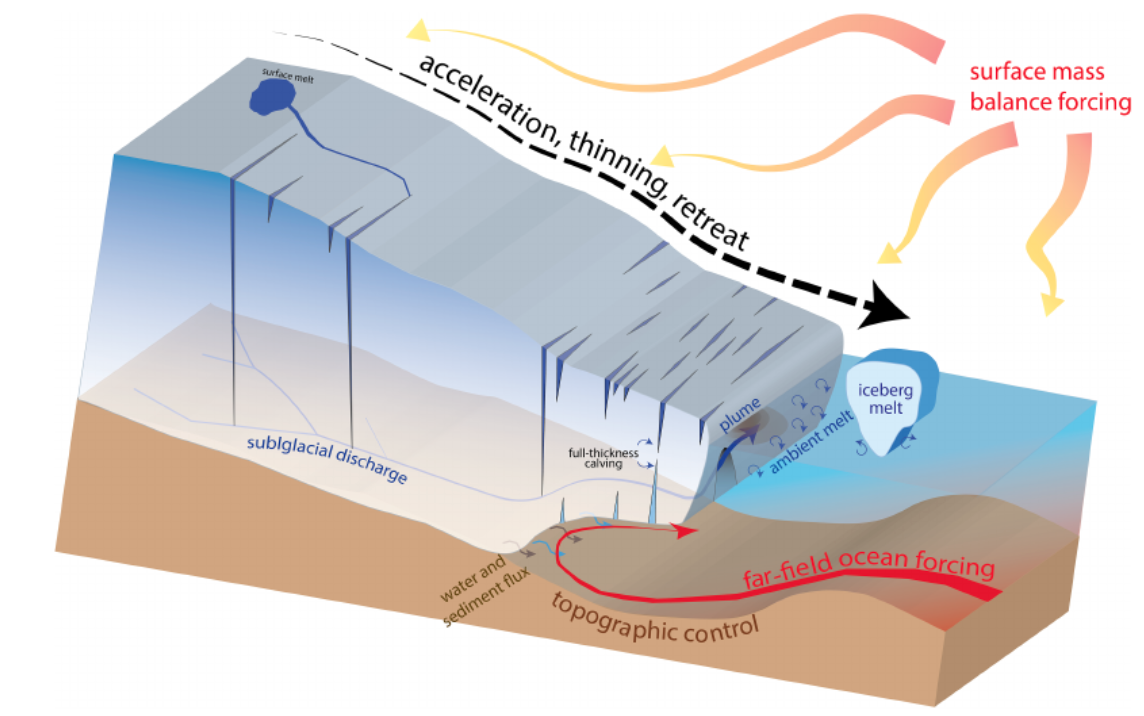
\includegraphics[width=10.2cm]{diagram.png}
	    \caption{Source \cite{catania2020future}. Conceptual diagram of outlet glacier processes that play in the terminal zone where the atmosphere, ice sheet, bedding and ocean interact. The red arrow indicates ocean thermal forcing occurring at depth in the fjords. The black arrow indicates that dynamic changes in outlet glaciers are more pronounced toward the end of the glacier. The blue arrows indicate subglacial water, which rises at the submarine terminus and rises along the end face, carrying sediment and nutrients with it (brown arrows). Subglacial plumes, melting icebergs, and distant ocean circulation all influence the circulation in the fjords \citep{catania2020future}.}
	\end{figure}
	
	%The mass balance of ice sheets, glaciers that have marine termini is partially determined by the interaction between ice and ocean \citep{jenkins2011convection}, and the region where that interaction occurs might include the base and front of a floating extension of the grounded ice.
	According to \citep{jenkins2011convection}, the region where the interaction between the ice and ocean occurs might include the base and front of a floating extension of the grounded ice. Different authors have done many works to understand some of the processes in ice-ocean interaction, ice base melting. \cite{jenkins2011convection} studied the convection-driven melting near the grounding lines of ice shelves and tidewater glaciers. The focus of their work was on the plumes generated by the meltwater from the ice shelves. \cite{kerr2015dissolution}, and \cite{gayen2016simulation} worked on the convection at the vertical ice face dissolving where the focus was on the buoyancy-controlled dissolving. \cite{gayen2016simulation} solved the Navier-Stokes equations for turbulent flow at a vertical ice-ocean interface at a scale similar to that obtained in the laboratory using Direct Numerical Simulations. They found good agreement with \cite{kerr2015dissolution} experiments, consistent with buoyancy controlling the width of the interfacial sublayer. The basal ice melting is a significant component of mass loss from the Antarctic ice sheet \citep{pritchard484mr, malyarenko2020synthesis}. However, projections of Antarctic contributions under future warming global and regional climate scenarios have significantly higher uncertainty due to poorly understood processes that could lead to rapid ice melting or discharge \citep{weertman1974stability,deconto2016contribution,gwyther2020vertical}. Therefore, more studies have to be done to understand basal melting better, address the uncertainty in current contributions, and improve future projections of Antarctic contributions.
	
	\cite{jenkins2011convection} emphasized that most melting estimates near the ice shelf grounding line have been based on observations of ice flux. Also, on the assumption of a steady-state, calculated melting or freezing and known surface ablation or accumulation balance the convergence or divergence of ice flux. Results suggest melt rates ranging from a few meters to a few tens of meters per year, with peak either at the grounding line or a short distance downstream \citep{jenkins1991ice,rignot2002rapid,jenkins2011convection}. Melting of the vertical calving front of a tidewater glacier is more challenging to observe; however, the net supply of meltwater to the ocean from observations of water properties in the fjord in front of LeConte Glacier front was melting at over 10 m per day \citep{motyka2003submarine}. Ocean circulation models under ice shelves can capture the large-scale characteristics of buoyancy-driven overturning circulation and reproduce the observed distribution of melting and freezing under ice shelves \citep{jenkins2002model, jenkins2011convection}. However, the resolution of all processes operating at the grounding line is generally beyond the capabilities of most ocean circulation models. 
	
	\section{Plume dynamics}
	Much of the meltwater from the ice sheets, glaciers, ice caps are discharged directly into the ocean at depth, generating buoyant plumes that move up the ice-ocean interface and merge with the surrounding ocean water \citep{hewitt2020subglacial}. The dynamics of these plumes are essential in regulating the heat transfer that drives submarine melt and controlling the depth to which glacial meltwater is exported to the open ocean. Therefore, they are crucial in the ice sheet response to ocean warming \citep{joughin2012ice, hewitt2020subglacial} and the ocean response to ice sheet melt \citep{straneo2013north}. 
	
		\begin{figure}[H]
	    \centering 
	    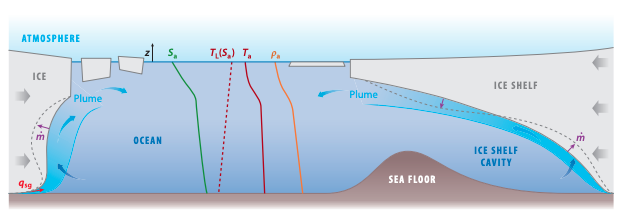
\includegraphics[width=15cm]{plume.png}
	    \caption{Source \cite{hewitt2020subglacial}. Plumes occur at the front of tidewater glaciers and beneath floating ice shelves. Subglacial discharge $q_{sg}$ (red arrow) and submarine melting $\dot{m}$ (purple arrows) produce buoyant water that rises up the ice front, entraining warmer ocean water. Typical profiles of ambient salinity $S_a\ (psu)$, temperature $T_a\ (^{\circ} C)$, and density $\rho_a\ (kg m^{-3})$, as well as liquidus $T_L(S_a)\ (^{\circ} C)$, are shown. The plume controls the melt rate and hence the shape of the ice–ocean interface. It can reach a level of neutral buoyancy and separate from the ice front, controlling the depth at which glacially modified water is exported to the open ocean \citep{hewitt2020subglacial}.}%. Decompression raises the freezing point so the plume can become supercooled, resulting in freeze-on of marine ice to the ice shelf base and creating cold waters that subsequently sink to produce Antarctic Bottom Water \citep{hewitt2020subglacial}.}
	    \label{fig:2}
	\end{figure}
	
	
	\noindent As depicted in figure $\ref{fig:2}$, the plumes form at the near-vertical front of tidewater glaciers and beneath relatively low-slope ice shelves. The former is typical of Greenland, while the latter is typical of the Antarctic ice sheet. According to \cite{hewitt2020subglacial}, on tidewater glaciers, melting driven by plumes affects the shape of the front; thus plays an essential role in the calving of icebergs. Under ice shelves, melting and freezing affect the shape of the ice shelf, which significantly affects the location of the grounded line.% and the flow of ice across it.
	
	Seawater in the vicinity of the ice is within a few degrees of freezing point and is a mixture of water of different origins and properties.  A common assumption is that the only source of buoyancy that acts to stratify the water column and drive the overturning circulation in the ice cavity is the generation of meltwater at the ice-seawater interface \citep{jenkins2011convection}. However, in a critical region such as Greenland, where outlet glaciers are grounded several hundred meters below sea level and terminate in a narrow fjord, freshwater will flow across the grounding line from the glacier bed. In Greenland, there are no direct observations of glaciers. However, theory and models indicate that the boundary layer is dominated by buoyant plumes driven by freshwater release from the surface melt at the ice sheet's base and from grounding line melt along the glacier face \citep{jenkins2011convection,straneo2013north}. For that reason, accurate mathematical representation of the ice-ocean boundary is crucial for understanding the key processes of the ice-ocean interaction and the impact of Greenland and Antartic ice loss on sea-level rise. 
	
	
	\begin{figure}[H]
	    \centering 
	    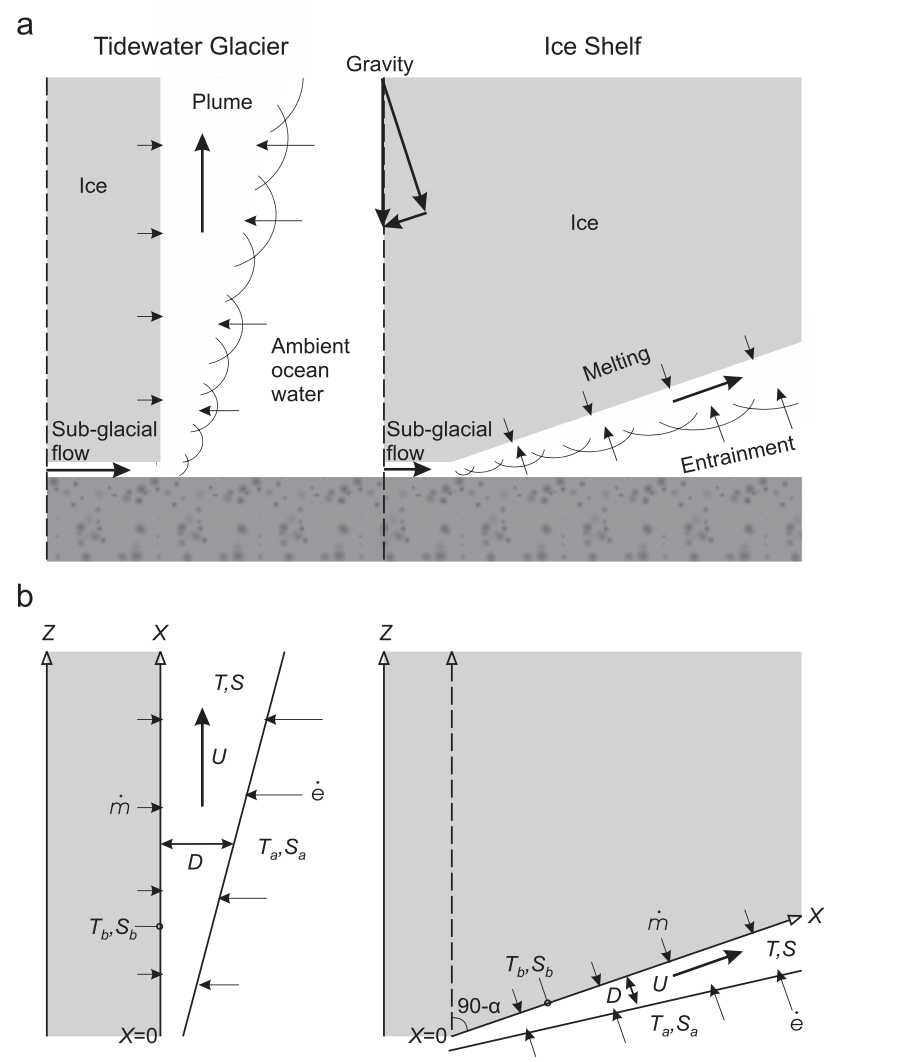
\includegraphics[width=12cm]{plumeD.png}
	    \caption{Source \cite{jenkins2011convection}. (a) Conceptual representation of a buoyant plume from freshwater flow at the grounding line of an ice shelf or tidewater glacier and (b) schematic picture of the numerical representation of (a) with the key variables defined. The plume rises on the ice face, entraining seawater in its way. The entrained seawater provides the heat that drives the melting of the ice face, and the meltwater thus derived adds to the buoyancy of the plume. Near the grounding line, most of the freshwater carried in the plume will be provided by subglacial flow, although freshwater provided by melt will dominate with sufficient downstream evolution \citep{jenkins2011convection}.}
	    \label{fig:3}
	\end{figure}
	
	
	
	Simple one-dimensional models can provide valuable insights and scaling arguments. Plume theory was initially developed by Morton et al. (1956) to study convection driven by point sources of buoyancy and then applied by Ellison and Turner (1959) in a slightly modified form to the case where buoyancy-driven flow is constrained to follow a solid boundary. MacAyeal (1985) was the first to apply this concept to large-scale circulation beneath ice shelves. According to \cite{jenkins2011convection}, the main characteristic of all plumes is that their volume flux increases with height by the entrainment of fluid from the surroundings. The approach presented here was used in the work of \citep{jenkins2011convection}. It accounts for all observed melting near the grounding lines. The only difference from previous applications is that the dominant source of buoyancy is defined by the initial conditions rather than the later evolution of the plume. The model describes mass, momentum, heat, and salt conservation and considers plume thickness $D\ (m)$, velocity $U\ (m\cdot s^{-1})$, salinity $S\ (psu)$, and temperature $T\ (^{\circ} C)$ as prognostic variables
	
	\begin{align*}
	    \dfrac{d}{dX}(DU)& = \dot{e} + \dot{m}\\
	    \dfrac{d}{dX}(DU^2)& = D\left(\dfrac{\rho_a-\rho}{\rho_0}\right)g\sin\alpha - C_dU^2\\
	    \dfrac{d}{dX}(DUT)& = \dot{e}T_a + \dot{m}T_b - C_d^{1/2}U\gamma_T(T-T_b),\\
	    \dfrac{d}{dX}(DUS)& = \dot{e}S_a + \dot{m}T_b - C_d^{1/2}U\gamma_S(S-T_b),\\
	\end{align*}
	
	\noindent where $\alpha$ is the angle of the ice shelf base from the horizontal, $\dot{m}\ (m\cdot s^{-1})$ is the melt rate, and the subscripts $a$ indicate conditions in the ambient water and $b$ conditions at the ice–ocean interface (see figure \ref{fig:3}). $\gamma_T\ (m\cdot s^{-1})$ and $\gamma_S\ (m\cdot s^{-1})$ is referred as temperature and salinity exchange velocity respectively, $\dot{e}$ is the entrainment rate. $C_d$ is a dimensionless drag coefficient, $\rho_a$ is the ambient water density, $\rho_0(kg\ m^{-3})$ is the reference density, and 
	$$\rho = \rho_0\left[1+\beta_S(S-S_a)-\beta_T(T-T_a)\right]$$ describe the equation of the state where $\beta_T$ is the coefficient of thermal expansion and $\beta_S$ is the coefficient of haline contraction. We will discuss about the melt rate, and the ice-ocean interface properties further in the following section.
	
	\cite{wells2008geophysical} also developed a detailed model for a plume rising along a vertical wall, suggesting two transitions. The first from a laminar state to a turbulent regime with a sublayer width set by the Rayleigh number $R_a = g'\delta^3/\kappa\nu$ with $g' = (\rho-\rho_0) g/\rho_0$ where $\rho\ (kgm^{-3})$ is the density, $g$ is the gravitational accelation and $\delta$ the molecular sublayer thickness. Then to a second turbulent regime with a sublayer width set by the shear stress of the turbulent external flow, determined by a critical Reynolds number, $R_e = U\delta/\nu$. Despite increasing applications on ocean forcing of glaciers in the past decades, they have not been able to cover the region near the grounding line. For example, the grounding line region, such as in the large vertical Tidewater glaciers of southwest and southeast Greenland, extends 5-10 km from the terminus due to vigorous calving, and the glaciers of northern Greenland, with ice tongues that extend several tens of kilometers. Thus, with no exception, these studies have failed to sample the ice-ocean boundary layer where the meltwater plume is expected to rise \citep{straneo2012characteristics}. However, it is possible to better understand the dynamics at the ice-ocean boundary by studying the transformation of ocean waters by the glacier in conjunction with thermodynamic models of ice melt in saline waters \citep{holland1999modeling}. This approach was recently applied in different studies (e.g. \cite{jenkins2011convection,gayen2016simulation,hewitt2020subglacial}).
	
	
	
	\section{Thermodynamic models of ice–ocean interaction}
	
    	The aim of modeling the ice-ocean interaction is to obtain a melt rate, interface temperature, and salinity at the ice interface  as realistic as possible. To determine the characteristics exactly, three physical constraints have to be considered. The interface must be at the freezing point, heat and salt must be conserved at the interface during any phase change \citep{holland1999modeling}.
        
        \subsection{Freezing point dependence}
        
    	The freezing point of seawater is a weakly nonlinear function of salinity and a linear function of pressure \citep{millero1978freezing}. %However, a linearized form is used in most of the studies to simplify the solution to the three-equations system obtain latter in this section. 
    	However, most studies use a linearized form to simplify the solution to the three-equation system obtained later in this section. The relationship between the temperature and salinity at the ice-ocean interface, $T_b\ (^{\circ}C)$ and $S_b\ (psu)$ is given by
		
		\begin{equation}
			\label{eq:1}
			T_b = \lambda_1 S_b+\lambda_2+\lambda_3p_b
		\end{equation}
		
		\noindent where $p_b\ (Pa)$ is the pressure at the interface and $\lambda_1\ (^{\circ}C\ psu^{-1}),\lambda_2\ (^{\circ}C),\lambda_3\ (^{\circ}C Pa^{-1})$ are constants. Equation $(\ref{eq:1})$ is valid only in the salinity range 4-40 psu and does not apply to pure freshwater \citep{holland1999modeling}.
		
		
		\subsection{Conservation of heat and salinity}
		
		The conservation of heat at the interface requires that the difference of the heat flux balances the source of latent heat resulting from ablation at the interface
		
		\begin{eqnarray}
			\label{eq:2}
			Q_i^T - Q_a^T = Q_{latent}^T,
		\end{eqnarray}
		
		\noindent where $Q_{latent}^T = -\rho_a\dot{m}L_i$ is the latent heat flux with $\rho_a\dot{m}$ representing the mass of ice that melted per unit time. $L_i\ (Jkg^{-1})$ is the specific latent heat of the ice. The heat flux at the interface in ice is given by $$Q_i^T = -\rho_i c_i\kappa_i^T\dfrac{\partial T_i}{\partial x},$$ and the heat flux at the interface in water is $$ Q_a^T = -\rho_a c_a\kappa_a^T\dfrac{\partial T_a}{\partial x},$$ 
		
		\noindent where $c_i\ (J /kg ^{\circ}C), c_a\ (J /kg ^{\circ} C)$ are the specific heat capacities of ice and ocean; $\kappa_i^T\ (m^2s^{-1}), \kappa_a^T\ (m^2s^{-1})$ are the thermal diffusivities of ice and seawater, and $\rho_i$ is the ice density. The heat conservation at the interface is then
		
		\begin{equation}
		\label{eq:3}
		    \rho_i c_i\kappa_i^T\dfrac{\partial T_i}{\partial x}\bigg|_b -\rho_a c_a\kappa_a^T\dfrac{\partial T_a}{\partial x}\bigg|_b = \rho_a \dot{m} L_i.
		\end{equation}
		
		\noindent Similarly, the conservation of salinity is given by
		
		\begin{equation}
			%\label{eq:4}
			Q_i^S - Q_a^S = Q^S_{brine},
		\end{equation}
		
		\noindent where $Q_{brine}^S = \rho_a\dot{m}(S_i-S_b)$ is the salt flux necessary to maintain the interface salinity at $S_b$. $Q_i^S$ is the diffusive salt flux into the ice, $S_i$ is  the salinity in the ice, and the salt flux in the water is $$Q_a^S = -\rho_a\kappa_a^S\dfrac{\partial S_a}{\partial x},$$ 
		\noindent where $\kappa_a^S$ is  the salinity diffusivity of the seawater.
		Considering both $Q_i^S$ and $S_i$ negligible \citep{oerter1992evidence,gayen2016simulation}, the salt conservation at the interface becomes 
		
		\begin{equation}
			\label{eq:5}
			\rho_a\kappa_a^s\dfrac{\partial S_a}{\partial x}\bigg|_b = \rho_a\dot{m}S_b.
		\end{equation}
		
		\noindent The equations $(\ref{eq:3})$ and $(\ref{eq:5})$ represent the boundary conditions at the ice-ocean interface. In some studies, the authors also neglect the heat flux into ice, $Q_i^T$ (eg. \cite{gayen2016simulation}). The boundary conditions are expressed in terms of melt rate $\dot{m}$, salinity, $S_b$ and temperature, $T_b$ at the boundary, thus we need to compute them in order to solve the boundary equations.
	
	    \subsection{Three-equation formulation}
		
		The three-equation formulation is one of the different approaches used to compute the melt rate, the interface temperature, and salinity. It divides the interface region into ice, the interface of ice-ocean, and the far-field ocean. It describes the conservation of heat equation and salt equation with fluxes across each boundary. This approach was developed by \cite{holland1999modeling} where the boundary layer is assumed to be laminar. Under this assumption the temperature and salinity would vary linearly between the interface and the mixed temperatures, so we have
		
		\begin{equation}
			Q_a^T = -\rho_a c_a\gamma_T(T_b-T_a),
		\end{equation}
		 and 
		 
		\begin{equation}
			Q_a^S = -\rho_a\gamma_S(S_b-S_a),
		\end{equation}
		
		\noindent where $\gamma_T$ and $\gamma_S$ is referred as temperature and salinity exchange velocity respectively. The exchange velocities can be either assumed constant or as function dependence on friction velocity, we refer to \citep{holland1999modeling} for their parameterization. The temperature gradient for the ice at the ice-ocean interface is given by
		
		\begin{equation}
			\label{eq:16}
			\dfrac{\partial T}{\partial x}\bigg|_b = \dfrac{\rho_a\dot{m}}{\rho_i\kappa_i^T}\left( T_i-T_b\right).
		\end{equation}
	
		By using the approximation of the heat and salt gradient at the interface, we obtain the three-equation formulation as
		
		\begin{align}
			T_b &= \lambda_1 S_b+\lambda_2+\lambda_3p_b,\\
			c_i\dot{m}\left(T_i-T_b\right) + c_a\gamma_T(T_a-T_b)& = \dot{m}L_i,\\
			\gamma_S(S_a-S_b) & = \dot{m}S_b.
		\end{align}
	
		\noindent After some algebra, we solve for $S_b$ and find that
		
		\begin{equation}
			AS_b^2 + BS_b + C = 0,
		\end{equation}
		
		\noindent where
		
	\begin{align*}
		A &= \lambda_1(c_a\gamma_T-c_i\gamma_S),\\
		B &= -c_a\gamma_T(T_a-\lambda_2-\lambda_3p_b) + c_i\gamma_S(T_i-\lambda_2-\lambda_3p_b+\lambda_1S_a)-\gamma_SL_i,\\
		C &= \gamma_SL_iS_a-c_i\gamma_SS_a(T_i-\lambda_2-\lambda_3p_b).
	\end{align*}
	
	Although the three-equation formulation is commonly used in recent studies (e.g. \cite{gayen2016simulation, gwyther2020vertical}) to model the oceanic flux at ice-ocean interface, various approaches have been adopted by some others authors. The one-equation formulation described by equation $(\ref{eq:1})$ has been used by (eg. \cite{jenkins1991ice,holland1998parameterization}) and its formulation is based on the fact that if the upper ocean layer relaxes to the freezing point instantaneously, there is no distinction between the properties of the interface and mixed layer. The disadvantage of using this approach come from the fact that the melting rate cannot be computed from the boundary condition. \cite{jenkins2010observation} and \cite{jenkins2011convection} used, the two-equation formulation define by 
	
	\begin{align}
			T_f & = \lambda_1 S+\lambda_2+\lambda_3p_b\\
			c_i\dot{m}\left(T_i-T_f\right) + c_a c_d^{1/2}\gamma_{TS}(T_a-T_f)& = \dot{m}L_i\\
	\end{align}
	
	\noindent where $T_f$ is the freezing temperature of the plume, and $c_d^{1/2}\gamma_{TS}$ is called Stanton number. \cite{jenkins2010observation} shows that the observation of water and melt properties at a Ronne Ice Shelf site can be fitted using either the three-equation or two-equation formulation.
	One advantage is its use to determine the melting rate.
	
	\begin{comment}
	To prescribed the boundary conditions at the ice face we revisited the conservation of salt and heat at the interface. In most of works done in the past, the boundary conditions at the ice-ocean interface are define as follows (e.g. \cite{gayen2016simulation}) where the heat flux through ice ($Q_i^T$) is neglected
	
	\begin{equation}
		\label{eq:eq10}
		\dfrac{\partial T}{\partial x}\bigg|_b = \dfrac{L_i}{\rho_ac_a\kappa_T}\dot{m}
	\end{equation}
	
	\noindent for the temperature and
	
	\begin{equation}
		\label{eq:eq11}
		\dfrac{\partial S}{\partial x}\bigg|_b = \dfrac{S_b}{\rho_a\kappa_S}\dot{m}
	\end{equation}
	
	\noindent for salinity. 
	
	\end{comment}
	
	Now, with the formula of the melt rate, temperature and salinity at the interface, the boundary conditions, equations $(\ref{eq:3})$ and $(\ref{eq:5})$ can be rewritten as follows by neglecting the heat flux into ice
	
	\begin{equation}
		\label{eq:eq10}
		\dfrac{\partial T}{\partial x}\bigg|_b = -\lambda_1T\bigg|_b + \lambda_1T_a, \quad \lambda_1 = \dfrac{\gamma_T}{\rho_a\kappa_T},
	\end{equation}
	
	\noindent for the temperature and 
	
	\begin{equation}
		\label{eq:eq11}
		\dfrac{\partial S}{\partial x}\bigg|_b = -\lambda_2S\bigg|_b + \lambda_2S_a, \quad \lambda_2 = \dfrac{\gamma_S}{\rho_a\kappa_S}.
	\end{equation}
	
	\noindent for salinity. The equations $(\ref{eq:eq10})$ and $(\ref{eq:eq11})$ represent the Robin boundary conditions.
	
	\section{Vertical ice face}
	
	There have been several studies on quantifying the melt rate in the region dominated by freshwater discharge \citep{wells2011melting, kerr2015dissolution, gayen2016simulation}.
     The melting rate depends not only on the thermal and salt diffusivities but also on the structure of the boundary layer. In the laminar regime, the melting rate is lower due to the thicker thermal boundary layer. At the same time, within the transition region, the interface temperature and melting rate increase rapidly with the rising plume \citep{gayen2016simulation}. \cite{kerr2015dissolution} in their work considered vertical ice adjacent to the ocean where the melting rate is controlled by the buoyancy-driven dissolving, and it is independent of the depth and plume velocity. They found in their analysis that the melting rate is 
	
	\begin{equation}
	    \dot{m} = constant\times (T_w-T_L)^{1.34},
	\end{equation}
	
	\noindent which is consistent with the theory prediction. The authors also pointed out that when the ambient temperature exceeds $3-4^{\circ} C$ above the freezing point temperature, a transition into turbulent melting is approached, and the interface temperature is overestimated. \cite{gayen2016simulation} solved the Navier-Stokes equations for turbulent flow at a vertical ice-water interface and found good agreement with the experiments of \cite{kerr2015dissolution}, consistent with buoyancy controlling the width of the interfacial sublayer. Another theoretical scaling for both vertical and horizontal boundaries suggests the existence of the second regime of turbulent natural convection at high Rayleigh numbers, the numbers associated with the buoyancy-driven flow that characterizes the flow regime ($R_a> 10^{16}$). In that regime, the thickness of the inner laminar boundary layer near the ice face is controlled by shear production rather than convective production of turbulence \citep{grossmann2000scaling, wells2008geophysical,kerr2015dissolution,gayen2016simulation}. \cite{mcconnochie2017using} found that for a vertical interface, the transition to a shear regime occurs at a plume speed of 3-5 cm/s. Such small-scale studies provide a unique opportunity to examine the ice-ocean interface and boundary layer development in a controlled environment, which field observations cannot achieve. However, these small-scale studies do not reach the Rayleigh numbers typically observed adjacent to an ice-ocean interface in the field \citep{malyarenko2020synthesis}. Therefore, further studies are needed in the examination of the vertical ice face, glaciers confined to fjords in complex geometries and the Antarctic glacier grounding line region.

	
	
	\section{Numerical Models}
	
	
	Numerical models that include the thermodynamic interaction between the ocean and the ice sheet are the best option for studying current and future Antarctic contributions to sea level (e.g. ROMS: \cite{dinniman2007influence}; MITgcm: \cite{losch2008modeling}; FESOM: \cite{timmermann2012ice}; COCO: \cite{kusahara2013modeling}; MPAS-O: \cite{ringler2013multi}; FVCOM: \cite{zhou2020modeling}).
	MPAS-O was developed base on finite-volume discretization of the incompressible Boussinesq equations \citep{ringler2013multi}.
	
	\begin{figure}[H]
	    \centering 
	    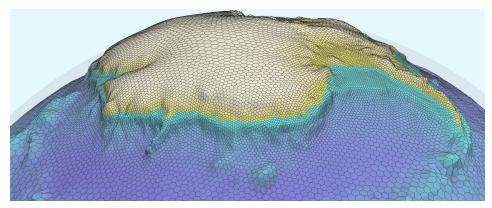
\includegraphics[width=13cm]{MPASg.png}
	    \caption{Source (\cite{MPAS}). Example of MPAS grids for the Southern Ocean and Antarctic Ice Sheet.}
	    \label{fig:4}
	\end{figure}
	
	\noindent In MPAS-O, accurate prediction requires acceptable ocean resolution to resolve the currents flowing around or under the ice shelves. Similarly, extremely high resolution, 1 km grid spacing (figure \ref{fig:4}) is required to accurately represent the transition between the grounded ice sheet and the floating ice sheet over Antarctica.
	
	Fully coupled ice sheet-ocean models will allow a comprehensive study of how ocean-driven basal melting affects Antarctica, but they are still in their infancy for large realistic domains. Therefore, the best current option is ice shelf-ocean models that neglect ice dynamics and assume steady-state ice geometry \citep{gwyther2020vertical}. These ice shelf-ocean models explore this data-deficient environment by simulating both small-scale processes and the large-scale spatial and temporal evolution of basal melting in Antarctica. In the recent study done by \cite{gwyther2020vertical} provides a test case for development of ice-ocean model applications; and better understand ice-ocean interactions. The study used three different modeling frameworks, the Regional Ocean Modeling System (ROMS), the Center for Climate System Research Ocean Component Model (COCO), and the Model for Predictions Across Scales: Ocean (MPAS-O).
	
	
	
	According to the results of \cite{gwyther2020vertical}, there are significant differences in the basal melting rate between these models, especially with COCO and MPAS compared to ROMS. Melting is lower in ROMS by a factor of two compared to COCO and MPAS-O. In addition, the ROMS model shows lower thermal entrainment (difference between the ambient ocean water temperature $T_a$ and the pressure freezing point $T_f$) across the ice shelf than COCO and MPAS-O models. According to the authors, the main reason for these results in ROMS is its higher vertical resolution. Their results also suggest a strong sensitivity of melt rates to the choice of vertical resolution, discretization, and boundary layer parameterization that could reasonably affect the sensitivity of the melt rate to changes in ocean forcing.  Many authors recognize the limitations of the current treatment of the ice-ocean boundary layer that results in a resolution dependence in melt rates. \cite{gwyther2020vertical} suggest that until the complete turbulent process can be solved explicitly, parameterizations of processes in the boundary layer will need to evolve with increased vertical resolution.
	
	Understanding the structure and mechanism that governs the thermodynamics and momentum exchange in the ice-ocean boundary layer is limited by the lack of observations and spatial non-uniformity of the ice-ocean interface. Given the non-uniformity of ice-ocean interactions and non-uniform ice melt, the ice face cannot be planar. Therefore, current numerical models developed based on finite difference, finite element, and finite volume methods lack of high-order algorithms and may not provide an appropriate approximation of the ice-ocean model at the ice face with complex geometry (figure \ref{fig:4}). Thus, the geophysical modeling community is exploring the spectral element method (SEM) approach to address the problems of multi-scale simulations in complex geometrical regions due to the geometric flexibility of their unstructured grids \citep{iskandarani2002multi}. It combines the geometric flexibility of low-order finite element methods with the high-order accuracy associated with spectral methods. 
	
	According to \cite{iskandarani2002multi} and \cite{ilicak2009non} the SEM method offers several advantages for geophysical simulations such as geometric flexibility with spatial discretization based on unstructured grids, high order convergence rates, dense computations at the element level leading to excellent scalability on parallel computers. Also SEM offers good convergence with the refinement of the elemental grid or increasing the order of the interpolation polynomial and has no significant numerical dissipation \citep{ilicak2009non}. The figure \ref{fig:5} depicts an example of a spectral element ocean model grid covering the majority of the global ocean. The unstructured grids nature gives the method its great geometrical flexibility and permits a better geometrical description of the complex ocean basins
	
	\begin{figure}[H]
	    \centering 
	    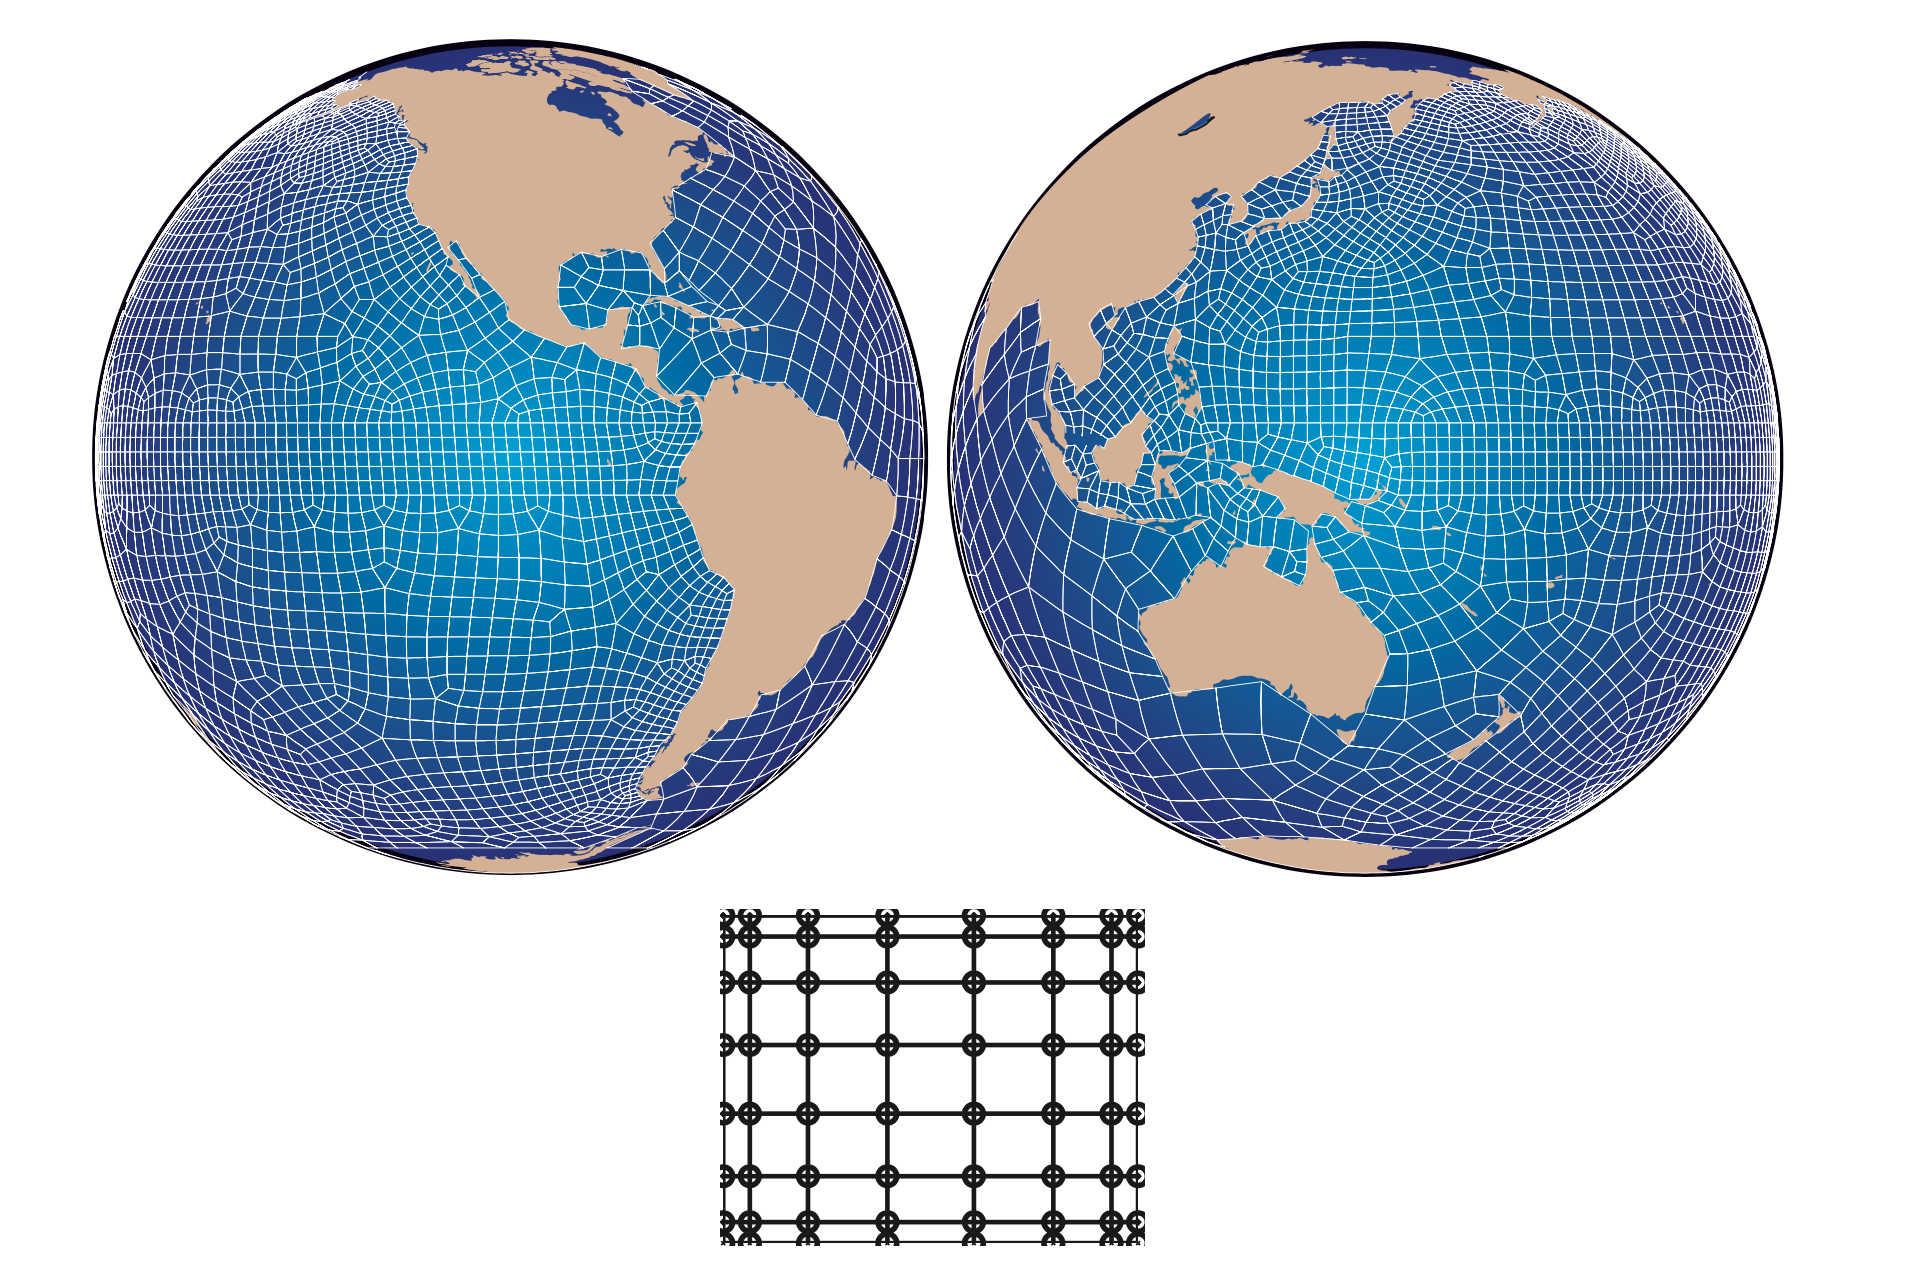
\includegraphics[width=13cm]{semGrid.png}
	    \caption{Source (\cite{iskandarani2002multi}). Elemental partition of the global ocean as seen from the eastern and western equatorial Pacific. The inset shows the element in the computational domain. The circles mark the interpolation points.}
	    \label{fig:5}
	\end{figure}
	
	
	
	%Thus, a model using spectral element method (SEM) can solve the problem of discretizing the ice interface. The SEM has some advantages in ocean modeling, which involves the complex interaction of stratified flows with topography  \citep{ilicak2009non}. The authors suggest that the SEM offers good convergence with the refinement of the elemental grid or increasing the order of the interpolation polynomial. The method has no significant numerical dissipation and offers geometric flexibility, especially for problems with complex geometry. Another advantage is the scalability of its code in parallel machines. 
	
	\cite{ilicak2009non} performed a large eddy simulation (LES) of the lock exchange problem using the non-hydrostatic spectral element model Nek5000. %The Nek5000 model is based on the SEM, which combines the high accuracy of spectral methods with the geometric flexibility of finite element methods. 
	Seven geometric cases with geometric deformations, including V-shaped and L-shaped deformations, which are typically observed in straits, are considered in the simulation. The results revealed significant differences in the amount of mixing between the different domain geometries. In particular, the L-shape leads to the highest level of mixing, and the lowest mixing is encountered in the V-shaped channel. The Nek5000 has also been used in the numerical simulation of bottom gravity currents, and the results have been useful to refine parameterizations of gravity current mixing for an ocean general circulation model \citep{chang2005comparison, ilicak2009non}. \cite{karniadakis1989spectral} also found that the SEM method can sustain the turbulent fluctuations flow. While the low-order schemes usually fail to maintain the turbulent fluctuations and force the flow to return to a laminar state. %From these results, SEM may help solve the geometry and high-order vertical resolution issues at the ice-ocean interface.
	From these results, SEM may be helpful to address geometry and high vertical resolution at the ice-ocean interface.

	
	
	\section{Limitations in ice-ocean interaction modeling}
	
    According to the papers used in this review, the numerical models have various limitations. Large-scale numerical models have not been able to cover the region near the grounding line, as in the case of the large vertical tidewater glaciers in Greenland, which extend 5-10 km from the terminus. Thus, without exception, these studies have failed to sample the ice-ocean boundary layer where the meltwater plume is expected to rise \citep{straneo2012characteristics}. Given the topography of the ice face, it will not be realistic to use most of the current models to access this topography. Similarly, it may be unrealistic for large-scale models to resolve plumes of the order of 10 m. Plume models assume a vertical ice front, but actual ice fronts have a more complicated geometry due to non-uniform submarine melt.
    In addition to the differences between numerical models depending on their framework, ice-ocean models, in general, are still subject to several limitations. Some of these are related to significant uncertainties in the ice face geometry and critical gaps in the knowledge of the dynamics at the ice-ocean interface, as \cite{mathiot2017explicit} highlighted in the case of the Nucleus for European Modeling of the Ocean (NEMO) framework.
    
    Improved predictions of the contribution of the glaciers, ice sheets, and sea ice melt to sea level rise require a better understanding of the processes that influence ice dynamics. The three-equation formulation that describes the thermodynamics of the ice-ocean interface assumes only vertical flows with no horizontal flows. However, \cite{jenkins2016simple} shows that an equilibrium state could be reached only in the boundary layer with a sloping interface and a buoyant plume if spatial gradients were present in properties such as temperature or horizontal velocity. The three-equation formulation has been applied to many ice-ocean models with different vertical configurations. The practical implementation of these parameterizations differs among model settings; thus, the results of ice-ocean simulations with different models may treat this vertical resolution dependence differently \citep{gwyther2020vertical}. Although the three-equation formulation has been used in many models and studies to quantify melt rate, observations of double diffusive staircases under the George VI ice shelf \citep{kimura2015estimation} are an illustration where it has been shown that the three-equation formulation does not accurately resolve melt rate. \cite{davis2019turbulence} showed that the wall law assumption inherent in the three-equation formulation does not hold at low flow rates.
    \section{Future Research Ideas}
    
    From the previous sections, we noticed that the current models for ice-ocean interaction have a limit in capturing the ice interface well, also the failure of the three-equation formulation in the double-diffusivity situation and flow of low rate. Therefore, further studies are needed to understand the physics and processes that govern that transfer of heat and salt from the ocean outside the boundary layer into ice face.
    Further work is needed to understand how plumes drive the detachment and calving of tidewater glaciers. Need to perform some  high-resolution modeling studies under a variety of basal conditions of the nature of turbulence and the rates of heat and salt transfer in the boundary layer. An open question is how ocean temperature, subglacial discharge, and ice dynamics control overall frontal melting rates. Another critical thing to think about is the formulation of the boundary conditions. In the three-equation formulation, the boundary values, temperature, and salinity are known, making the problem of Dirichlet conditions. Therefore, given the non-uniform melting of the ice face and the plume in the boundary layer must rise from the bottom to the top of the ice, it may be appropriate to consider other boundary conditions like Neumann or Robin. It would also be good to improve the three-equation formulation and include horizontal flows in the formulation. Develop a new ocean model of ice-ocean interaction based on spectral element method or the discontinuous Galerkin (DG) method because, in the DG method, the numerical solution can be discontinuous across element boundaries. The communication between elements is through the fluxes exchanged across the edges of the elements.


	%\newpage
	
	%\bibliographystyle{unsrt}

    %\bibliographystyle{apa}
	\bibliography{refComp}
	
	\end{document}